\documentclass[9pt,numbers,reprint]{sigplanconf}

\pdfoutput=1
\pdfminorversion=7

\newcommand{\ignore}[1]{}

\usepackage{fancyhdr}
\usepackage[normalem]{ulem}
\usepackage[hyphens]{url}
\usepackage{hyperref}

\usepackage{amssymb}
\usepackage{amsmath}
\usepackage{color}
\usepackage{graphicx}
\usepackage{minted}
\usemintedstyle{bw}

\usepackage{balance}
\usepackage{booktabs}
\usepackage{subcaption}
\usepackage{tikz}
% \usepackage{pgfplots}


\title{The Path to DPDK Speeds for AF\_XDP}

\authorinfo{Magnus Karlsson and Bj\"orn T\"opel}
           {Intel, Inc.\\Stockholm, Sweden}
           {\{magnus.karlsson,bjorn.topel\}@intel.com}


\begin{document}
\makeatletter
\def\@copyrightspace{\relax}
\makeatother

\maketitle

\begin{abstract}
AF\_XDP is a new socket type for raw frames introduced in Linux
4.18. The current code base offers throughput numbers around 20 Mpps
per application core for 64-byte packets on a typical Broadwell
server, however, not much effort was spent on optimizations. The focus
of this paper is the performance optimizations needed for AF\_XDP to
get it to the performance levels of user-space network driver packages
such as DPDK.

We present various optimizations that fall into two broad categories:
ones that are seamless to the application and ones that requires
additions to the uapi. With these optimizations, we show we can reach
our goal of close to 40 Mpps of throughput for 64-byte packets in
zero-copy mode for Rx and close to 70 Mpps for Tx. We end this paper
by presenting further possible optimizations that will bring the Rx
performance even higher.
\end{abstract}

\keywords
Networking, Linux, AF\_XDP, XDP, packet processing, zero-copy.

\section{Introduction}
In the beginning of August 2018, Linux 4.18 was released and with that
a new socket type was introduced called AF\_XDP. It is designed to
pass network traffic from the driver in the kernel up to user space as
fast and efficiently as possible, but still abiding by all the usual
robustness, isolation and security properties that Linux provides. The
performance target of AF\_XDP has always been to be close to that of
software packages with user space drivers (full or partial) and/or
zero-copy semantics such as DPDK~\cite{dpdk}, Netmap~\cite{netmap},
and PF\_RING~\cite{pfring}. The initial release of AF\_XDP in 4.18
targeted basic functionality and was not optimized for
performance. While it did deliver quite good throughput performance
between 15 and 22 Mpps~\cite{af_xdp_patch, af_xdp_patch_zc,
  af_xdp_patch_i40e, af_xdp_lwn} for the benchmarks in the sample
application, this is only around 50\% or less of what the techniques
above can deliver. And this is not enough.

In this paper, we present a number of optimization to AF\_XDP that
takes the performance up to levels that are closer to or even on par
with what user-space driver techniques, such as DPDK, can
deliver. With these optimizations, more than double the throughput
performance: from 15 Mpps to 39 Mpps for Rx and from 25 Mpps to 68
Mpps for Tx. We have limited the optimization proposals to patch sets
that we believe are acceptable to the networking community and
non-intrusive to other component with the exception of XDP~\cite{xdp}
in some cases, as AF\_XDP uses XDP for its Rx data path.

To improve the performance of the Rx path, we propose three sets of
improvements:
\begin{itemize}

\item Optimize the XDP path and XDP driver implementation for the post
  Spectre world with retpolines~\cite{retpoline}. A performance drop
  of nearly 50\% for XDP has been reported~\cite{jesper_xdp_perf_drop}
  and as AF\_XDP uses XDP, we suffer from this too. This patch set
  optimizes indirect calls and switch statements in the data path so
  that they perform better with retpolines.

\item Introduce a new {\tt bind} option in which the user does not
  have to supply an XDP program and all traffic on the specified queue
  id is sent up to the socket. This is realized in AF\_XDP by loading
  a built-in XDP program and this program and the path leading up to
  it can be optimized leading to substantial performance
  improvements. Another benefit with this is that it improves ease of
  use and adoption of AF\_XDP as an external XDP program is no longer
  required the configuration path becomes simpler.

\item Introduce an execution context in the XDP code instead of using
  per-cpu state. While this improves performance on its own, more
  importantly, it becomes possible to implement a number of other
  performance improvements based on having information more readily
  available.

\end{itemize}

To reach these performance levels on the Tx side, we propose four new
patch sets:
\begin{itemize}

\item Allow for multiple Tx sockets to be connected to one umem, so
  that we can spread the Tx load over multiple Tx HW queues. This
  patch is also required to support QoS and shaping features in NICs,
  as this usually requires one queue per class. So this feature is
  useful even without the performance improvements it gives rise to.

\item Extend the driver so that AF\_XDP gets its own HW queue. In the
  upstream version, XDP and AF\_XDP shares one HW queue, but by
  giving AF\_XDP its own queue we can make the Tx completion code much
  more efficient.

\item Change the batch size and descriptor queue sizes in the user mode
  application. We have now tuned these to the new higher throughput
  levels. But note, that they are kept the same for all experiments,
  so we are not fine tuning anything.

\item Introduce a new {\tt setsockopt} that queries the device if the NIC
  supports in-order completion and if so stops using the completion
  queue and signals completions using the tail pointer of the Tx ring
  instead. This cuts down the coherency traffic between the user mode
  application on one core and the softirq processing on another core
  and also gets rid of the backpressure mechanism between the
  completion ring and the associated Tx rings.

\end{itemize}

When AF\_XDP is executed, two cores are used: one for the user mode
application and one for the Rx/Tx processing in kernel space. But with
user-mode driver models, such as DPDK, the application and driver is
usually executed on the same core. They can do that as both
application and driver reside in the same program. This can give rise
to a large performance increase since it eliminates the coherency
traffic between the cores in the two core setup. If we co-located the
application and kernel driver to the same core with AF\_XDP, there
would be extensive mode and context switching between the two and
performance would be poor even though we eliminated all coherency
traffic. But there is a way to execute a networking application with
AF\_XDP using only a single core and not have to do any context switching
between the application thread and any ksoftirqd thread, and that is
by using \emph{busy poll()}~\cite{busy_poll} ({\tt POLL\_BUSY\_LOOP}) in
conjunction with AF\_XDP.

With busy poll(), the network driver is driven by the user space
application through the poll() syscall, in contrast to the normal case
where it is driven asynchronously by interrupts fired by the NIC. The
driver is executed in the same context as the application, thus
we do not require any context switching and the application and driver
can be executed on the same core. The added overhead is the poll
syscall and its associated mode switch into the kernel to execute the
driver. With busy poll we get 30 Mpps for Rx and 51 Mpps for Tx,
compared to 39 Mpps and 68 Mpps with the normal setup without busy
poll. But note that the busy poll results are with a single core while
the other results are with two, so if you look are what you get per
core, the busy poll results are better.

In summary, the results look promising and make the performance of
AF\_XDP to be much closer to or even on par with user-space driver
models. We will try to get these patches into mainline during the next
12 months. But even though we believe the performance is now in the
``good enough'' territory for a number of interesting applications
using 40 Gbit/s devices, there are still many more performance
optimizations that could be done, and should be, to cater for upcoming
100 Gbit/s and 200 Gbit/s network devices and applications with even
higher performance requirements.

This paper is outlined as follows. In section \ref{sec:afxdp}, we
first present the basics of AF\_XDP followed by the proposed
optimizations in section \ref{sec:opt}. Section \ref{sec:exp:meth}
deals with the experimental methodology followed by the experimental
results in section \ref{sec:exp:res}. The paper is ended (sections
\ref{sec:future}, \ref{sec:conclutions} and \ref{sec:thanks}) with
some discussions and future work and finally the conclusions.


\section{AF\_XDP}
\label{sec:afxdp}

AF\_XDP was designed to be able to deliver raw packets from networking
cards (\emph{NIC}) to a user space process with a performance
comparable to solutions such as DPDK~\cite{dpdk},
Netmap~\cite{netmap}, and PF\_RING~\cite{pfring}. As AF\_XDP is built
as an extension to \emph{XDP} (eXpress Data Path)~\cite{xdp}, we need
to explain some of its features first to see how AF\_XDP builds on top
of it.

\begin{figure}[ht]
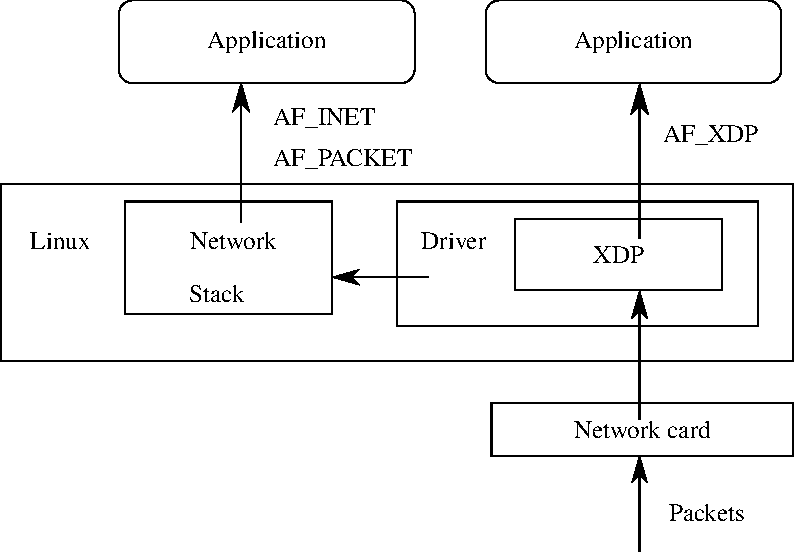
\includegraphics[width=.48\textwidth]{xdp.pdf}
\caption{XDP can process special user space applications in the kernel
  driver. AF\_XDP is the mechanism for which XDP can directly redirect
  packets up to an application in user-space with zero-copy semantics.}
\label{fig:xdp}
\end{figure}

XDP is a layer inside a Linux networking driver that for each packet
will execute a piece of validated code loaded from
user-space. This piece of code will then take actions on each
packet. These actions are (somewhat simplified) to \emph{drop} the
packet, to \emph{pass} it to the Linux networking stack or to
\emph{transmit} it out the same ({\tt XDP\_TX}) or another networking
interface ({\tt XDP\_REDIRECT}) as seen in Figure~\ref{fig:xdp}. As the XDP
program is executed in the driver, it can take these actions
very quickly. But as the program is limited in size, there are only
a limited set of actions that can be performed in XDP and if more complex
processing is need, the packet can be passed on to the Linux stack and
perhaps even up to user space through one of the many socket types
available such as raw sockets (AF\_PACKET) or regular TCP/IP ones
(AF\_INET).

AF\_XDP is a new socket type that permits raw packet data from the NIC
to be delivered straight to user space from XDP without any copying
and at significantly higher speeds than before~\cite{af_packet_v4}. It
compares most closely with AF\_PACKET in that it delivers raw packets
to user space, however, it does so without sending a copy of the
packet through the networking stack as it is zero-copy. AF\_XDP works
in three different modes from slowest to fastest: skb mode that works
on any NIC, XDP copy mode that works on any NIC with XDP support in
the driver, and zero-copy mode that only works on XDP enabled drivers
that have been extended to support zero-copy mode. In this paper, we
will only consider zero-copy mode as it has the best performance.

The XDP program decides to which AF\_XDP socket the packet should be
sent to. The sockets are put in the new XSKMAP map type and the XDP
program can then pick which entry in this map a packet should be sent
to. As XDP is a highly flexible program, the possible load balancing
schemes for AF\_XDP are also very flexible. Anything you can run in
XDP is possibility. For better performance, but less flexibility, you
can use HW steering in the NIC instead. But note that in the current
code base, an XDP program is mandatory even when you have HW steering.

\begin{figure*}[ht]
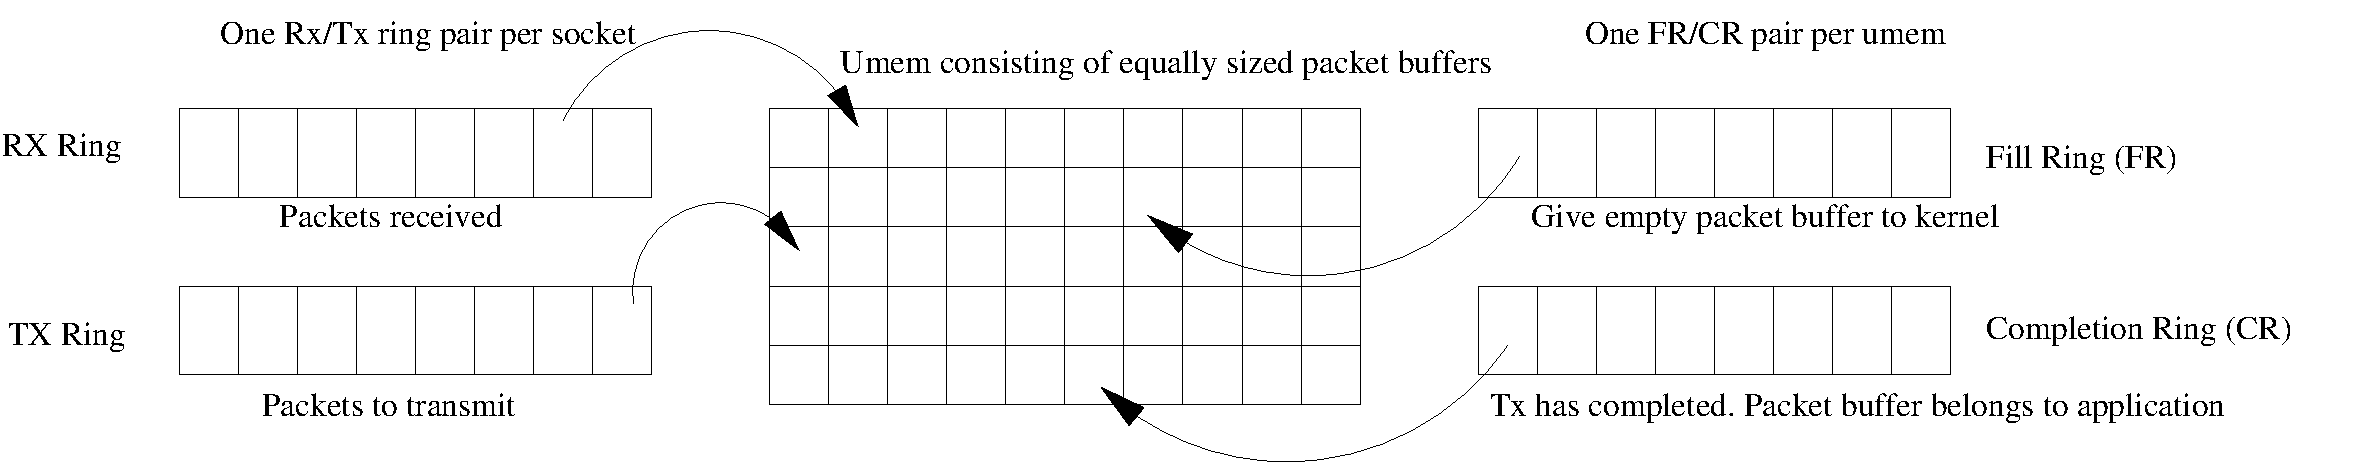
\includegraphics[width=\textwidth]{queues_and_umem.pdf}
  \caption{The four rings of AF\_XDP and the umem containing all the
    packet buffers.}
  \label{fig:queues_and_umem}
\end{figure*}

From the application program point of view, all packets are located in
an application allocated memory area called \emph{umem} as seen in
Figure~\ref{fig:queues_and_umem}. This is an area of equally sized
chunks of memory called \emph{packet buffers} in which packets can
reside. Associated with a umem comes two rings: the \emph{fill ring}
and the \emph{completion ring}. The fill ring is used to transfer
ownership of a packet buffer from user space to the kernel, and
conversely the completion buffer signals that ownership of a packet
buffer has been transferred from the kernel to user space. The
application indicates what packet buffer to transfer ownership of by
putting the address of that packet buffer into the fill ring. Note,
that this is the relative address from the start of the packet buffer,
not the actual virtual address. In the same way, the kernel indicates
ownership transfers in the completion ring by entering the relative
address of the desired packet buffer into it.

\begin{listing}[ht]
\begin{minted}[xleftmargin=9pt,fontsize=\scriptsize,tabsize=2]{c}
/* Rx/Tx descriptor */
struct xdp_desc {
        __u64 addr;
        __u32 len;
        __u32 options;
};

/* Fill/Completion descriptor */
__u64 addr;
\end{minted}
\caption{The descriptors of the Rx, Tx, Fill, and Completion rings.}
\label{lst:desc_structs}
\end{listing}

Now we have a way to transfer ownership of packet buffers without
sending or receiving any data. To be able to send and receive packet data, we
need two more rings: the \emph{Rx ring} and the \emph{Tx ring}. As
seen in Listing~\ref{lst:desc_structs}, the descriptor format of these
are larger than the fill and completion rings. When a packet is
received, the kernel fills in a descriptor in the Rx ring, signifying
what packet buffer contains the packet data by setting addr to the
relative address of the packet buffer and indicating its
length in len. There is also an options field, but it is reserved for
future extensions. By checking the Rx ring, an application can find
out if it has received a packet. Conversely, if the application wants
to send a packet, it puts the same kind of information in the Tx
ring, signaling to the kernel that this packet should be
transmitted. Note that the Rx and Tx rings belong to the socket and
each socket is bound to one umem which has only one fill ring and one
completion ring. But many sockets can be bound to the same umem as
long as they are bound to the same network device and queue id. In
that case, there will be many Rx/Tx ring pairs.

A typical life-of-a-packet for AF\_XDP is the following. A packet
enters the NIC and the Linux driver picks it up, executes the XDP
program that decides if the packet should be sent to a specific AF\_XDP
socket. As AF\_XDP is executing in zero-copy mode, the NIC has already put
the packet in a packet buffer in the umem area so the only thing the
kernel has to do is fill in the Rx descriptor to tell the application
where this new packet resides and the length of it. The application
will then check the Rx ring if it has received any packets. Once it
has finished processing the packet, it can return it to the kernel via
the fill ring so that a new packet can arrive in that packet buffer.

Tx works in a similar way but using the Tx and completion rings. When
the application wants to send a packet, it fills out the next available
descriptor in the Tx ring to point to the packet buffer it wants to
send. The kernel will then pick up this request and send it to the
hardware. Once the hardware has sent the packet, the kernel signals
that it has indeed sent the packet by returning the packet buffer to
the application via the completion ring.

\begin{listing}[ht]
\centering
\begin{minted}[xleftmargin=9pt,fontsize=\scriptsize,tabsize=2]{c}
sfd = socket(PF_XDP, SOCK_RAW, 0);

start_of_umem = malloc(size_of_umem);
mr.addr = start_of_umem;
mr.len = length_of_umem;
mr.chunk_size = 2048;
mr.headroom = headroom;
setsockopt(fd, SOL_XDP, XDP_UMEM_REG, &mr, sizeof(mr));

size = nr_descs_in_fill_queue;
ret = setsockopt(sfd, SOL_XDP, XDP_UMEM_FILL_RING,
                &size, sizeof(size));
size = nr_descs_in_completion_queue;
ret = setsockopt(sfd, SOL_XDP, XDP_UMEM_COMPLETION_RING,
                &size, sizeof(size));

size = nr_descs_in_rx_queue;
ret = setsockopt(sfd, SOL_XDP, XDP_RX_RING,
                &size, sizeof(size));
size = nr_descs_in_tx_queue;
ret = setsockopt(sfd, SOL_XDP, XDP_TX_RING,
                &size, sizeof(size));

/* Get the structure of the queues */
getsockopt(sfd, SOL_XDP, XDP_MMAP_OFFSETS, &off, &optlen);

fill_q = mmap(NULL, off.fr.desc * nr_descs_in_fill_queue *
                sizeof(u64),
                PROT_READ | PROT_WRITE,
                MAP_SHARED | MAP_POPULATE,
                sfd, XDP_UMEM_PGOFF_FILL_RING);
/* ...and so on for all four queues */

sxdp.sxdp_family = PF_XDP;
sxdp.sxdp_ifindex = if_nametoindex(interface_name);
sxdp.sxdp_queue_id = queue_id;
bind(sfd, (struct sockaddr *)&sxdp, sizeof(sxdp));
\end{minted}
\caption{The control path of AF\_XDP in C-style pseudo-code.}
\label{lst:ctrl_path}
\end{listing}

Listing~\ref{lst:ctrl_path} shows the control path in
pseudo-code. First we have to create an AF\_XDP socket through the
usual socket() call. After that some memory is allocated for the umem
and register it through the {\tt setsockopt} option {\tt
  XDP\_UMEM\_REG}. The four rings are then created with the {\tt
  setsockopt}s {\tt XDP\_RX\_RING}, {\tt XDP\_TX\_RING}, {\tt
  XDP\_UMEM\_FILL\_RING}, and {\tt XDP\_UMEM\_COMPLETION\_RING}. The
application then has to ask the kernel for the structure of these
rings using the {\tt setsockopt} {\tt XDP\_MAP\_OFFSETS}. The reason
for this is that the ring structures are highly optimized to minimize
cache coherency traffic and might look different on various
architectures. Now we have created all the structures we need and are
ready to start receiving and/or sending traffic from a network device
and this is indicated by issuing a {\tt bind()} call providing the
interface as well as the queue id of that interface from which we
would like to receive traffic from and/or transmit traffic on. This
concludes the control path of the set up.

\begin{listing}[ht]
\begin{minted}[xleftmargin=9pt,fontsize=\scriptsize,tabsize=2]{c}
void process_batch(void)
{
    struct xdp_desc descs[BATCH_SIZE];

    rcvd = xq_deq(rx, descs, BATCH_SIZE);
    if (!rcvd)
        return;

    for (i = 0; i < rcvd; i++) {
        char *pkt = xq_get_data(descs[i].addr);
        process_packet(pkt, descs[i].len);
    }

    umem_fill_to_kernel(fq, descs, rcvd);
}

/* Run-to-completion model */
while (1) {
    process_batch();
}

/* With poll() */
fds[0].fd = sfd;
fds[0].events = POLLIN;

while (1) {
    ret = poll(fds, 1, 0);
    if (ret <= 0)
       continue;

    if (fds[0].fd != sfd ||
        !(fds[0].revents & POLLOUT))
       continue;

    process_batch();
}
\end{minted}
\caption{The Rx data path of AF\_XDP in C-style pseudo-code.}
\label{lst:rx_data_path}
\end{listing}

The data path is simpler and is shown in
Listing~\ref{lst:rx_data_path}. It comes in two main flavors: either a
run-to-completion-model or by calling {\tt poll()} (or {\tt select()},
{\tt epoll()}, etc) to receive a packet. In the run-to-completion
model, the application just busy polls the Rx ring in order to check
if it has received a message. Once it receives a batch, it goes on to
process them. In the {\tt poll()} model, it calls poll when it has
nothing to do, and when poll returns there is either a packet to
receive or a timeout has occurred.

\begin{listing}[ht]
\begin{minted}[xleftmargin=9pt,fontsize=\scriptsize,tabsize=2]{c}
static struct xdp_desc descs[BATCH_SIZE];

int send_batch(descs)
{
    u64 comp_descs[BATCH_SIZE];

    if (xq_nb_free(tx, BATCH_SIZE) >= BATCH_SIZE)
       xq_enq(tx, descs, BATCH_SIZE) == 0);
    else
       return 0;

    sendto(sfd, NULL, 0, MSG_DONTWAIT, NULL, 0);
    rcvd = umem_complete_from_kernel(cq,
                                     comp_descs,
                                     BATCH_SIZE);
    if (rcvd > 0)
       process_completions(descs, rcvd);

    return rcvd;
}

/* Run-to-completion model */
while (1) {
    produce_packets(descs);
    (void)send_batch();
}

/* With poll() */
fds[0].fd = sfd;
fds[0].events = POLLOUT;

while (1) {
    produce_packets(descs);
    nr_pkts_sent = send_batch();

    if (nr_pkts_sent == 0) {
       ret = poll(fds, 1, 0);
    }
}
\end{minted}
\caption{The Tx data path of AF\_XDP in C-style pseudo-code.}
\label{lst:tx_data_path}
\end{listing}

For the Tx path shown in Listing~\ref{lst:tx_data_path}, a descriptor
for the packet to be sent is put in the Tx ring. The kernel can pick
this up to send it in two ways: either through a sendmsg() syscall
from the application or through the transmit path NAPI context that
might already be running. If the Tx ring is full, the application can
call poll() to wait for the ring to have one or more free entries so
that a packet can be sent, or just poll continuously using the
run-to-completion model. The Tx code also needs to check the completion
ring in order to be able to reuse packet buffers once the kernel has
sent them.

\begin{figure}[ht]
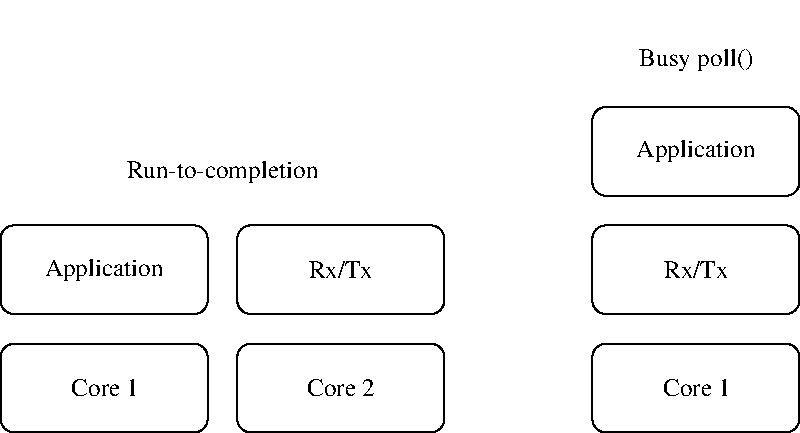
\includegraphics[width=.48\textwidth]{two_vs_one_core.pdf}
\caption{When run normally, AF\_XDP will consume two cores in our
  experiments, but if busy poll() support is used both application and
  Rx/Tx processing can run efficiently on a single core.}
\label{fig:two_vs_one_core}
\end{figure}

When an AF\_XDP program executes it usually consumes two cores: one
for the application and one for ksoftirqd executing the Rx and Tx
processing in a NAPI context as seen to the left in
Figure~\ref{fig:two_vs_one_core}. If the driver performs Rx and Tx
processing in different NAPI contexts, then they can execute on
different cores for a total of three cores. But this is not the case
for the driver we are using in our experimental evaluation. This is in
contrast with DPDK and other user-mode driver packages which can, with
good performance, execute both Rx/Tx processing and the application on
a single core. If we did this, the performance would drop by orders of
magnitude due to context switching. But there is a solution for this
in Linux and that is to use the \emph{busy poll()} support ({\tt
  BUSY\_POLL\_LOOP}) in the kernel. With this feature, and the
corresponding enablement in the AF\_XDP code, only one core is needed
as the application will drive the NAPI context from the poll()
syscall. With this busy poll() support, we can achieve a set up that
is similar to DPDK, if desired. We will evaluate this support in the
results section.

AF\_XDP was introduced in Linux 4.18 and the source code can be found
in the net/xdp directory and the headers in \texttt{include/net/} {\tt
  xdp\_sock.h}. Note that some of the Rx path is in the XDP path and
that code is in \texttt{net/core/filter.c}. An example sample program
can be found in \texttt{samples/bpf/xdpsock\_user.c} and the XDP
program used to route the packets are in
\texttt{samples/bpf/} {\tt xdpsock\_kern.c}.


\section{Optimizations}
\label{sec:opt}

This section presents the proposed optimizations that require some
changes to non AF\_XDP components and/or can generate architectural
design discussions. The optimizations that we think are trivial are
not mentioned here. Instead they will be mentioned briefly in the
results section.


\subsection{Built-In XDP Program}

In the current code base, it is mandatory to install an XDP program
that routes packets to one or more AF\_XDP sockets. Without this
program, the AF\_XDP sockets will not receive any traffic at all. But
when the application writer only wants to use the simplest possible
XDP program that sends all packets from a queue id to a single socket
bound to that queue id, we propose to provide a built-in XDP program
that the user does not have to load. This will nearly half the amount
of setup code required for an XDP program. More importantly for this
paper, if we provide this built-in XDP program, we can implement a
faster path through the XDP code up to the AF\_XDP code that
significantly improves performance for this simple case.

We propose to add this support by adding a new flag to the {\tt bind} call
called {\tt XDP\_ATTACH}. When this flag is set, the AF\_XDP code will load a
built-in XDP program for you. This XDP program behaves like an
ordinary XDP program: you can dump it or replace it with
another XDP program on top of it. A change that we would like to
propose is that this built-in XDP program forms a hitch with any
regular, loaded XDP program. If an XDP program is loaded on top of the
built-in, the externally loaded program will replace the built-in
one. But if the externally loaded XDP program is unloaded, then the
built-in program will become active again. The reason for this is that
we think this is a good way to get it back. Another option would have
been to just have no XDP program running once the external one is
unloaded (as it is today), but in that case we would have to kill all
sockets on that interface and restart them to get traffic back or
provide a new XDP program with the basic functionality, but that would
defeat the whole purpose of this optimization.

We envision that at least one more built-in program would be useful
in the future and that would be an XDP program that copies the packet
and passes the copy to the Linux stack and the original to user
space. This could be used by applications that today use AF\_PACKET
such as tcpdump, wireshark and some DPI applications.


\subsection{Retpoline Optimizations}

The retpoline mechanism that mitigates Spectre v2 type of attacks can
cut the performance of XDP by up to
50\%~\cite{jesper_xdp_perf_drop}. As AF\_XDP is based on XDP, it has
a negative effect on it too, but only for the Rx part as the Tx part
does not use the XDP Tx code at this point in time. Retpoline degrades
the performance of indirect function calls, so that is something we
would like to avoid.

The built in XDP program that was introduced in the previous section
can be used to cut down the number of indirect function calls in the
XDP path as we now know exactly what path it will take and that this
program will not be replaced under our feet. We also optimized the XDP
path in the NIC driver by replacing switch statements on the
XDP actions with if statements, as the switch statements generated
jump tables with indirect function calls.


\subsection{XDP Optimizations}

One more optimization we tried on the XDP Rx path was to replace the
per-cpu state with an explicit context that is passed between
functions. While this makes the function calls longer (and uglier), it
provides a number of performance benefits. Retrieving data from the
stack allocated explicit state is cheap compared to using the per-cpu
state. This explicit context is also used to cut down the number of
look-ups in the XDP code, which also improves performance.


\subsection{Multiple Tx Rings for one umem}

In applications that use QoS and shaping support present in many NICs,
it is important to support multiple Tx sockets bound to different
queue ids but the same umem. Each one of these sockets will then be
treated differently by the NIC according to the QoS and shaping set
up. One example of such an area is the radio access and core network
of the mobile phone infrastructure. It is not uncommon to have more
than 10 classes of service in these systems since a lot of the traffic
goes over pay per use, shared transport networks. We also also
observed that spreading the Tx load over multiple queues increased
performance

This feature can be supported without any extensions or changes to the
uapi. Tx-only sockets can now be bound to a umem that has other
sockets and queue ids bound to it. But note that there can still only
be one Rx ring id associated with the umem. In order to preserve the
Single-Producer Single-Consumer semantics of the rings, the AF\_XDP
code will ask the driver if it can support this mutual exclusion by
for example running the handling of the rings in the same NAPI
context or by some HW mechanism. If so, this is left up to the
driver. If the driver replies no, then the synchronization will occur
in the AF\_XDP code using a spinlock which is usually more expensive,
but will work for any driver.


\subsection{In-Order Completion}

\begin{figure}[t]
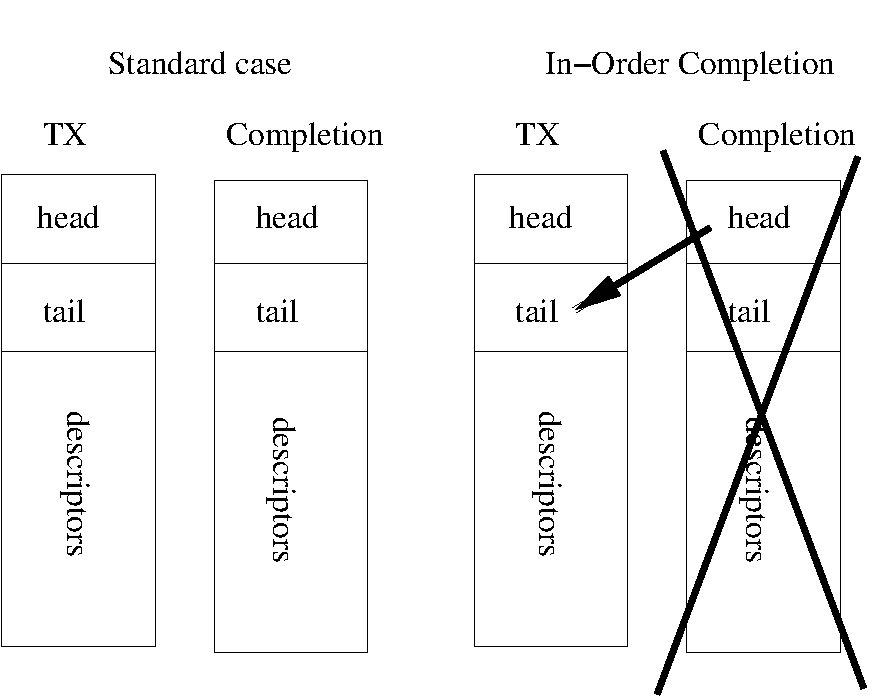
\includegraphics[width=.48\textwidth]{in_order.pdf}
\caption{Normally, the head pointer in the completion ring signals
  that packet buffers have completed and which one have to be read out
from the completion ring itself. With the in-order optimization, the
completion ring can be skipped completely and the tail pointer in the
Tx ring will now signify completions in the same order as in the Tx ring.}
\label{fig:in_order}
\end{figure}

The current uapi assumes that completions can be delivered
out-of-order by the underlying NIC and AF\_XDP code. That is the reason
why there is a completion ring with entries stating what packet
buffers that have completed. But what if the NIC can only deliver
packets in-order? In that case we actually do not need the completion
ring entries as they would be in the exact same order as the entries
in the Tx ring, as seen in Figure~\ref{fig:in_order}. We only need a
mechanism to signal that entries up to a certain point in the Tx ring
have completed, and that can be done with the tail pointer of the Tx
ring.

To support this feature, we introduce a new {\tt setsockopt} called
{\tt XDP\_INORDER\_COMPLETION}. When called it will return an error
code if in-order completion cannot be guaranteed by the driver and 0
if it can be supported. In that case, the application only needs to
check the Tx ring and can completely ignore the completion ring. It
does not even have to exist. From a performance perspective, not
having to populate or use the completion ring cuts the amount of
coherency traffic between the two cores. We can also stop running the
backpressure mechanism between the completion ring and the Tx
ring. This mechanism guarantees that there is always space in the
completion ring once we send a packet to the NIC, so that we do not
have to buffer anything in our code path. But without the completion
ring, there is no need for this, cutting down the coherency traffic
even further.


\subsection{Busy Poll() for AF\_XDP}

During the past couple of years, a number of people have added busy
poll() support~\cite{busy_poll} to poll(), epoll() and select(). In
this mode, the NAPI context associated with receiving and sending
messages to and from a socket can be driven by the syscall
itself. This happens if the NAPI context is not already running
because it has gotten for example an interrupt.

The main advantage of busy poll() is that we can run the application
and its associated Rx and Tx actions on a single core as depicted in
Figure~\ref{fig:two_vs_one_core}. This will eliminate the coherency
traffic between the two cores completely but the cost of this is the
poll syscall itself that we do not need to use in the
run-to-completion model that uses two cores.


\section{Experimental Methodology}
\label{sec:exp:meth}

We run on a dual socket system with two Broadwell E5-2660 @ 2.7 GHz
with hyper-threading turned off. Each socket has 14 cores which gives a
total of 28. The memory is DDR4 @ 2133 MT/s (1067 MHz) and the size of
each DIMM is 8192MB and with 8 of those DIMMs in the system we have 64
GB of total memory. We run Linux version v4.19-rc6-2008-g438363c0feb8
from the bpf-next tree with all Meltdown and Spectre mitigations
turned on. The distribution we use is Ubuntu 18.04.1 LTS, and the
compiler used is gcc version 7.3.0. We use two Intel I40E 40Gbit/s
networking cards version 2.3.2-k with firmware version 6.01. Only a
single interface/port is used on the card but we use two queues on
each interface (in all experiments except the first one in the Tx
section). Both NICs are served by the same core. The BIOS is from
Intel and has version number GRRFCRB1.86B.0261.R01.1507240936 and the
microcode has signature 0x000406f0. Power save has been turned off to
provide more stable performance numbers. All the four types of HW
prefetchers are turned on. Packets are generated by commercial packet
generator HW that is generating 64-byte packets at full 40 Gbit/s line
rate to each NIC.

The micro-benchmarks used in this study are shown in Table
\ref{table:benchmarks}. All of them are part of the xdpsock\_user.c
sample application. Rxdrop and txpush does not touch packet data
while l2fwd touches every packet by swapping the MAC addresses. Each
benchmark runs for 60 seconds and each application process executes on
its own core with cpu affinity. All processes are run on the same
socket as the NIC is plugged into.

\begin{table}[ht]
\centering
\begin{tabular}{|c|p{5.5cm}|} \hline
\textbf{Benchmark} & \textbf{Description} \\ \hline
rxdrop & RX only without packet data touch\\ \hline
txpush & TX only without packet data touch\\ \hline
l2fwd & RX + swap MAC headers + TX\\ \hline
\end{tabular}
\caption{The micro-benchmarks used in this paper.}
\label{table:benchmarks}
\end{table}

For the DPDK experiments, we use the same system and kernel as for the
AF\_XDP experiments. We use DPDK version 18.08 and compile it using
the standard supplied options and that is without any retpoline
support. We use both vectorized and scalar drivers in the
experiments. The same two NICs are used with two queues active on a
single port per NIC. We use the DPDK I40E PMD with 32-byte descriptors
as that is what is used in the Linux driver, however both DPDK and
AF\_XDP will get a performance boost (2\% for DPDK) by moving to
16-byte descriptors. But this has not been implemented in the Linux
driver. The testpmd application is used for all benchmarks and the
command line is \texttt{testpmd -l 14-15 -n 4 -w 0000:81:00.1 -w
  0000:86:00.0 -- -i --portmask=0x3 --rxd=512\\  --txd=512 --txq=1
  --rxq=1} and the prompts that follows for the different applications
can be found in Table~\ref{table:dpdk_commands}. We modified the
txonly code to use pregenerated packets to improve its performance and
to make it comparable to the AF\_XDP txonly that also uses
pregenerated packets\footnote{Performance results are based on testing
  as of October 17, 2018 and may not reflect all publicly available
  security updates. See configuration disclosure for details. No
  product can be absolutely secure.}.

\begin{table}[ht]
\centering
\begin{tabular}{|c|c|} \hline
\textbf{Benchmark} & \textbf{Testpmd Command Line} \\ \hline
rxdrop & set fwd rxonly\\ \hline
txpush & set fwd txonly\\ \hline
l2fwd & set fwd macswap\\ \hline
\end{tabular}
\caption{The DPDK testpmd command lines used for the benchmarks in
  this paper.}
\label{table:dpdk_commands}
\end{table}


\section{Experimental Results}
\label{sec:exp:res}

This section starts by first reporting the results of the Rx
optimizations in section \ref{sec:exp:rxres}, followed by the Tx
optimizations in section \ref{sec:exp:txres}. We then put all the
optimizations together when the results for the busy poll()
implementation are reported in section \ref{sec:exp:combres}. In
section \ref{sec:exp:xdpres}, we show how the optimizations improve
the performance of the XDP path and finally section
\ref{sec:exp:dpdkres} compares AF\_XDP's performance to DPDK's.


\subsection{RX Results}
\label{sec:exp:rxres}


Figure~\ref{fig:results_rx} shows the results of the proposed Rx
optimizations. ``Baseline'' refers to the performance of the code
without any of our optimizations in it, what you would get if you
would compile the latest bpf-next or net-next tree.  ``XDP\_ATTACH''
introduces the {\tt XDP\_ATTACH} option and by doing that we can use a
simpler built-in XDP program that gives rise to faster {\tt
  xdp\_do\_redirect}, {\tt xdp\_do\_flush\_map} and a specialized
version of {\tt bpf\_redirect\_map} called {\tt bpf\_xsk\_redirect}
that improves performance. The next two categories are self
explanatory, but the ``various driver opts'' inlines a number of
functions in the data path of the driver, restructures struct to be
more cache friendly, increases the tail bump interval from 32 to 128
and other optimizations. The ``Explcit context in XDP path'' was
explained in it own section.

\begin{figure}[ht]
\centering
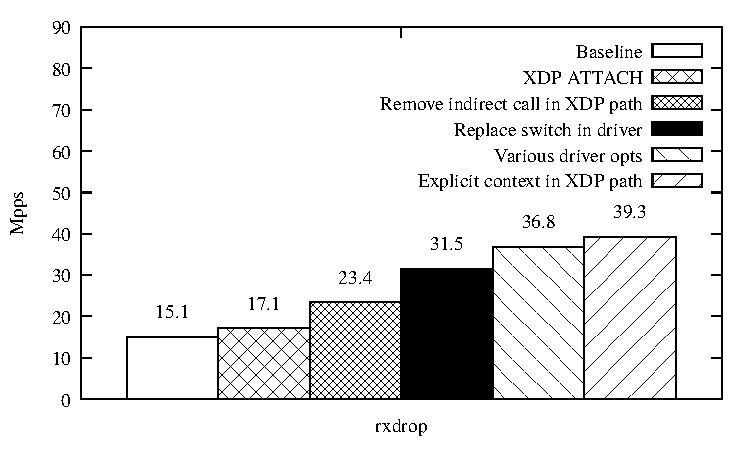
\includegraphics[width=.5\textwidth]{results_rx.pdf}
\caption{Results for rxdrop and the various Rx optimizations.}
\label{fig:results_rx}
\end{figure}

As can be seen the performance after all the optimizations is
increased by 131\% from 15.1 Mpps to 39.3 Mpps. This is mainly due to
the shorter code path that can be gained by the built-in XDP program
and especially by the retpoline optimizations.


\subsection{TX Results}
\label{sec:exp:txres}

Figure~\ref{fig:results_tx} shows the results of the proposed Tx
optimizations. ``Baseline'' is the same build as the one for Rx,
while ``Batch size and descriptor changes'' is when the batch
size of the application is increased from 16 to 64 and the ring sizes
are increased from 1024 to 2048. The other ones should be self
explanatory and/or covered in the optimization section.

\begin{figure}[ht]
\centering
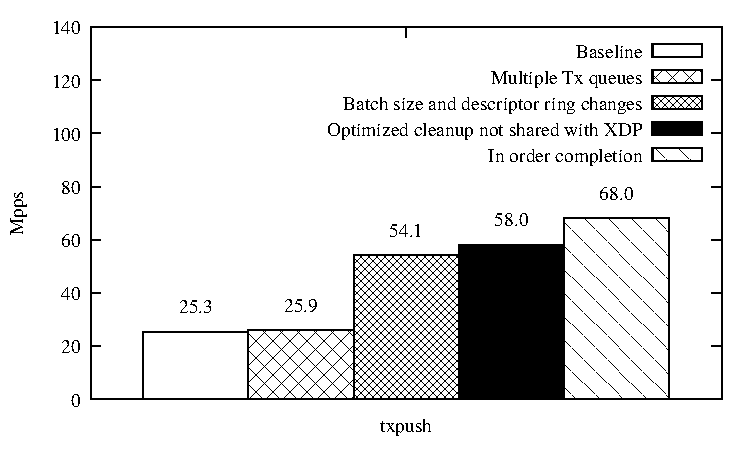
\includegraphics[width=.5\textwidth]{results_tx.pdf}
\caption{Results for txpush and the various Tx optimizations.}
\label{fig:results_tx}
\end{figure}

From the figure, we can see that the performance is increased by 169\%
or from 25.3 Mpps to 68.0 Mpps with all the Tx optimizations. (Note
that we can get more than 59.5 Mpps because we are using two 40 Gbit/s
NIC cards.) The highest performance gain is found by just tuning the sample
application slightly. We had not given this much love before, but by
just increasing the batch size and ring sizes we could gain a
substantial performance increase. Without the prior optimizations,
increasing these would not have matered that much. It is the
cumulative effect of all three optimizations that is seen here. The
in-order completion mode can increase the throughput even more up to
68.0 Mpps.


\subsection{Combined Results and Busy Poll()}
\label{sec:exp:combres}

Figure~\ref{fig:results_poll} shows a comparison between the
run-to-completion model that we have used in the experiments so far
and using the poll() syscall in the busy poll() mode. The main
difference between these modes is that the first mode uses two cores,
one for the application and one for Rx/Tx processing, while the busy
poll() mode uses only one core driving both the application and all
Rx/Tx processing in a manner much more similar to a typical DPDK
setup. All the Rx and Tx optimizations from the previous sections are
used in these measurements.

\begin{figure}[ht]
\centering
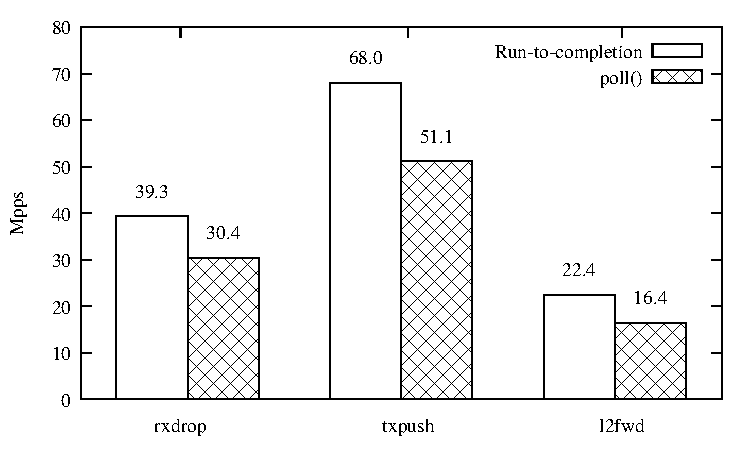
\includegraphics[width=.5\textwidth]{results_poll.pdf}
\caption{Results with and without busy poll(). Note that
  run-to-completion uses two cores but busy poll() only one.}
\label{fig:results_poll}
\end{figure}

As can be seen from the results, busy poll() decreases the performance
by between 20\% and 25\%. But note that busy poll() only uses a single
core instead of two (one fully loaded Rx/Tx core and a very lightly
loaded application core), so on a per core basis the performance of
busy poll() is between 50\% and 59\% better than the run-to-completion
model. This is mainly due to the fact that we do not have to
communicate any data between cores since it is all local to a single
core and this eliminates any coherency traffic leading to better
performance. The performance drawback with busy poll() is that incurrs
a system call overhead for the poll() call itself. This is something
that the run-to-completion model avoids as it directly polls the
relevant rings without any system call. But it is good to
be able to pick between both these models. There are workloads and
systems where one would be preferable to the other. E.g., for
multi-stage pipelined workloads, using several cores for just
application processing makes sense. But a workload for which the
packets can be easily distributed between cores by a NIC, the
busy poll() model is usually a better fit.


\subsection{XDP Results}
\label{sec:exp:xdpres}

\begin{figure*}[ht]
\centering
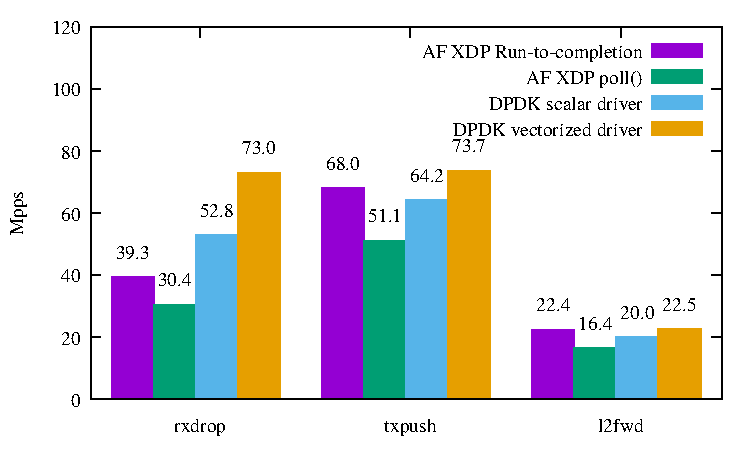
\includegraphics{results_dpdk.pdf}
\caption{Results comparing AF\_XDP with DPDK for three micro benchmarks.}
\label{fig:results_dpdk}
\end{figure*}

% \input{results_dpdk.tex}

Some of the performance improvements we made to AF\_XDP are also
beneficial to the regular XDP path. Table~\ref{table:results_xdp}
shows the performance increase of the xdp\_drop micro-benchmark found
in the \texttt{samples/bpf} directory in Linux. This benchmark when run
with the notouch option is the same as rxdrop but implemented in
XDP. As can be seen from the table, the throughput is increased by
23\%. So our optimizations of AF\_XDP that touches the XDP path has
not decreased the performance. On the contrary.

\begin{table}[ht]
\centering
\begin{tabular}{|c|c|c|} \hline
\textbf{Benchmark} & \textbf{Before} & \textbf{After optimizations} \\ \hline
xdp\_drop & 19.9 & 24.5 \\ \hline
\end{tabular}
\caption{The performance improvement to XDP as a result of the AF\_XDP
  targeted optimizations in this paper.}
\label{table:results_xdp}
\end{table}


\subsection{Comparison with DPDK}
\label{sec:exp:dpdkres}

The benchmark for highly optimized drivers and SW interfaces for
packet processing is today DPDK~\cite{dpdk}. It is frequently used
together with switching software to show really high throughput
numbers in the range of 1 Tbit/s worth of
switching~\cite{fdio_one_tbits}. The question is then, how does
AF\_XDP with these new set of optimizations compare to DPDK?

Figure~\ref{fig:results_dpdk} shows the performance of AF\_XDP and
DPDK for three benchmarks: rxdrop, txpush and l2fwd. For DPDK we have
used both scalar drivers (not using any vector or floating point
instructions) and vectorized drivers. As far as we know, there are no
vectorized networking drivers available in Linux at the time of
writing.

In summary, when we compare the busy poll() mode, that uses the same
amount of cores as DPDK, to DPDK with scalar drivers then AF\_XDP is
only around half the performance of DPDK. The run-to-completion mode
fares better and is even faster than DPDK (running a scalar driver)
for Tx but around 30\% slower for Rx. So we need to put more effort in
optimizing the Rx path and the busy poll() path. More interestingly,
when we actually start to touch the data in l2fwd, which is the normal
case for pretty much all non toy-applications, the difference between
AF\_XDP and DPDK becomes much smaller. The run-to-completion mode of
AF\_XDP is faster than the scalar DPDK driver but slower than the
vectorized one and busy poll() is only 16\% slower when both DPDK and
AF\_XDP are running scalar drivers. The more we actually use the data,
the less the performance difference will be. It would be interesting
to evaluate the performance difference for some real workloads and see
how they compare and where we need to focus our efforts. What we have
here are just micro-benchmarks.

We can also see from the results that vectorized drivers do offer a
performance boost, between 12\% and 38\% for the DPDK micro-benchmarks
used in this paper. The question is how much performance increase this
translates to for realistic workloads and if this increase offsets the
lowered maintainability and flexibility of such drivers.


\section{Future Work and Discussion}
\label{sec:future}

It is clear from the feedback we have gotten from initial users that
the setup and data plane usage of AF\_XDP needs to become simpler to
lower the bar of entry. Currently, it seems that users are just
copying the code from the sample program, which is not a good solution
in the mid to long term. The {\tt XSK\_ATTACH} optimization presented
in this paper is the way we propose to facilitate the setup of an
AF\_XDP socket, but to make the data path simpler to use, we need
something else. We would like to propose to add a lean and mean access
library for AF\_XDP sockets to libbpf, in the same manner as XDP has
added helper functions to facilitate adoption. This could present a
libc interface (or at least libc-like) to the user with familiar
functions such as {\tt recv, recvmsg,} and {\tt sendmsg}. This would
go well with the control plane usage of pure libc functions and the
already existing usage of {\tt poll, select} and {\tt sendto} in the
data plane. This library could then also be used to implement a really
simple DPDK PMD for AF\_XDP.

It would be beneficial to add hugepage support to AF\_XDP, not only
because it will cut down the TLB miss rate, but more so because it can
cut down the communication rate on the fill ring. In the fill ring we
indicate which page buffers should be returned by indicating what
chunk it belongs to. In the current implementation the chunk size can
be 2K or 4K, but with huge pages this could be for example 64K. So
indicating the ownership transfer of 32 consecutive 2K page buffers to
the kernel can be accomplished with just one write to the fill ring
when the chunk size is 64K, instead of 32 writes with a chunk size of
2K. This should improve performance.

Another avenue worth pursuing is to optimize the driver for ``XDP
first''. Currently we use the standard skb path, but there are many
things in that path that cannot happen because they are not supported
in XDP or AF\_XDP. We could, for example, register a special NAPI
handler that only deals with XDP Rx and/or Tx rings and provide a slim
and highly optimized path from there. Another example would be to go
to 16-byte descriptors for those queues as these can be handled faster
by the I40E NIC and also consumes less memory which could lead to
better performance.

One idea that we had for this paper, but had no time to implement, was
to batch the XDP processing so that a batch of packets is first
received, then that batch is processed in the XDP program and their
corresponding actions recorded, then after this the actions are
performed as a batch. When we implemented AF\_PACKET V4, we
experimented with this and it provided better throughput as it used
the instruction cache more efficiently. But we have not had the time
to implement this in the latest Linux kernel with AF\_XDP. Jesper
Dangaard Brouer has also posted interesting
suggestions~\cite{jesper_batching} on how to batch more in XDP.

We would like to encourage users out there to try out AF\_XDP on real
commercial workloads to see how it performs instead of our
micro-benchmarks that we have gotten. Please report any performance
problems, bugs and improvement suggestions on the mailing list so that
we can address them.


\section{Conclusions}
\label{sec:conclutions}

This paper presented a number of possible performance optimizations to
both the Rx and Tx paths of AF\_XDP. Most of them are transparent to
the user with the exception of the {\tt XSK\_ATTACH} {\tt bind} option
and the {\tt XSK\_INORDER\_COMPLETION} {\tt setsockopt} extension that
require application changes to take advantage of them.

The performance evaluation shows that the performance compared to the
current baseline in bpf-next and net-next is improved by 160\% from
15.1 Mpps to 39.3 Mpps for Rx and by 169\% or from 25.3 Mpps to 68.0
Mpps for Tx. We also evaluate the support of the busy poll() feature
in conjunction with AF\_XDP and while it reduces the total performance
by between 20\% and 25\%, it also cuts down the number of used cores
to one. Measured on a per core basis, busy poll() actually increases
performance with another 50\% compared to the optimized Rx and Tx
results. We also compare AF\_XDP against DPDK and while there is still
substantial work required on the Rx side to reach the same performance
levels, Tx and an application that actually touches the data, l2fwd,
offers comparable performance to DPDK when we run in run-to-completion
mode.


\section{Acknowledgments}
\label{sec:thanks}

We would really like to thank the reviewers on the mailing list and
all the people that have taken AF\_XDP for a spin and reported issues,
bugs and improvement suggestions: Ilias Apalodimas, Daniel Borkmann,
Jesper Dangaard Brouer, Willem De Bruijn, Eric Dumazet, Alexander
Duyck, Mykyta Iziumtsev, Jakub Kicinski, Song Liu, David S. Miller,
Sridhar Samudrala, Yonghong Song, Alexei Starovoitov, William Tu, Anil
Vasudevan, Jingjing Wu, and Qi Zhang. We owe you one.

\bibliographystyle{abbrvnat}
\bibliography{bibliography}


\end{document}
